% !TeX encoding = UTF-8
% !TeX program = xelatex+bibtex
% !TeX spellcheck = LaTeX

% Author : Shlw

\documentclass[UTF-8]{beamer}

\usepackage{graphicx}
\usepackage{ctex}
\usepackage{amsmath,amssymb,amsfonts}
\usepackage{multicol}
\usepackage{bm}
\usepackage{extarrows}
\usepackage[ruled]{algorithm2e}
\usepackage{hyperref}
\usepackage{comment}
\usepackage{xifthen}
\usepackage{tikz,mathpazo}


\usetikzlibrary{shapes.geometric, arrows}
\tikzstyle{startstop} = [rectangle, rounded corners, minimum width=2.5cm, minimum height=1cm,text centered, draw=black, fill=red!30, font=\bf]
\tikzstyle{io} = [trapezium, trapezium left angle=70, trapezium right angle=110, minimum width=3cm, minimum height=1cm, text centered, draw=black, fill=blue!30, font=\bf]
\tikzstyle{process} = [rectangle, minimum width=3cm, minimum height=1cm, text centered, draw=black, fill=orange!30, font=\bf]
\tikzstyle{decision} = [diamond, minimum width=2.5cm, minimum height=1cm, text centered, draw=black, fill=green!30, font=\bf]
\tikzstyle{arrow} = [thick,->,>= stealth]
\tikzstyle{line} = [thick]

\newcommand\ppar[1]{\left( #1 \right)}
\newcommand\abs[1]{\vert #1 \vert}
\newcommand\frpar[1]{\left\lfloor #1 \right\rfloor}
\newcommand\clpar[1]{\left\lceil #1 \right\rceil}
\setbeamertemplate{footline}[frame number]

\useoutertheme{sidebar}
\useoutertheme{infolines}
\useinnertheme{circles}
\usefonttheme{professionalfonts}
\bibliographystyle{plain}
\hypersetup{hidelinks}

\definecolor{pkured}{HTML}{94070A}
\colorlet{pkuredgray}{pkured!75!gray}
\colorlet{pkuredblack}{pkured!50!black}
\definecolor{nonpkublue}{HTML}{03356B}
\definecolor{nonpkugreen}{HTML}{025709}
\definecolor{nonpkupurple}{HTML}{9370DB}

\setbeamercolor{structure}{fg=pkured}
\setbeamercolor{normal text}{fg=black,bg=white}
\setbeamercolor{alerted text}{fg=nonpkugreen!67!yellow,bg=white}
\setbeamercolor{example text}{fg=nonpkublue,bg=white}
\setbeamercolor{palette primary}{fg=pkuredblack,bg=gray!20}
\setbeamercolor{palette secondary}{fg=pkuredblack,bg=pkuredgray!20}
\setbeamercolor{palette tertiary}{fg=gray!10,bg=pkured!90}
\setbeamercolor{palette quaternary}{fg=gray!10,bg=pkured}
\setbeamercolor{titlelike}{parent=palette quaternary}
\setbeamercolor{frametitle}{fg=gray!10}
\setbeamercolor{block title}{fg=gray!10,bg=pkured}
\setbeamercolor{block title alerted}{use=alerted text,fg=gray!10,bg=nonpkugreen!75!bg}
\setbeamercolor{block title example}{use=example text,fg=gray!10,bg=nonpkublue!75!bg}
\setbeamercolor{block body}{parent=normal text,use=block title,bg=block title.bg!25!bg}
\setbeamercolor{block body alerted}{parent=normal text,use=block title alerted,bg=block title alerted.bg!25!bg}
\setbeamercolor{block body example}{parent=normal text,use=block title example,bg=block title example.bg!25!bg}
\setbeamercolor{sidebar}{bg=pkured!90}
\setbeamercolor{palette sidebar primary}{fg=gray!10}
\setbeamercolor{palette sidebar secondary}{fg=pkured!20}
\setbeamercolor{palette sidebar tertiary}{fg=pkured!20}
\setbeamercolor{palette sidebar quaternary}{fg=gray!10}
\setbeamercolor*{separation line}{}
\setbeamercolor*{fine separation line}{}

\newenvironment{red}[1][]
{\ifthenelse{\isempty{#1}}
{\begin{block}{\vspace{0.2em}}}
{\begin{block}{#1}}}
{\end{block}}

\newenvironment{blue}[1][]
{\ifthenelse{\isempty{#1}}
{\begin{exampleblock}{\vspace{0.2em}}}
{\begin{exampleblock}{#1}}}
{\end{exampleblock}}

\newenvironment{green}[1][]
{\ifthenelse{\isempty{#1}}
{\begin{alertblock}{\vspace{0.2em}}}
{\begin{alertblock}{#1}}}
{\end{alertblock}}

\newcommand{\mygraph}[2]{
\begin{figure}[H]
  \centering
  \includegraphics[width=0.6\textwidth]{#1}
  \caption{#2}
\end{figure}
}

\title{Progressive Photon Mapping}
\author{吴克文\ 梁家硕}
\date{2017年6月}

\begin{document}
\frame{\titlepage}

\begin{frame}
\tableofcontents
\end{frame}

\section{PPM\ vs\ PM}
\frame{\sectionpage}
\begin{frame}
\begin{blue}[Why Progressive Photon Mapping]
Photon Mapping作为全局光照领域的主流算法,以其高效率,能处理多种光照效果%
等特点,一直受到广泛的关注。\\\pause
然而,Photon Mapping算法的一个主要问题在于,使用光子进行光能估计的过程引入%
了偏差。理论上,要完全消除偏差,需要存储无穷的光子,这从计算机存储角度来看%
是不可接受的。\\\pause
为此,Toshiya Hachisuka提出了Progressive Photon Mapping(又称渐进式%
光子映射),采用多遍的绘制流程,通过不断向场景中发射光子达到不断减小偏差的%
目的,亦解决了Photon Mapping的存储问题。
\end{blue}
\end{frame}

\section{效果展示}
\frame{\sectionpage}
\frame{\mygraph{box2}{PPM原作者的场景}}
\frame{\mygraph{specular}{镜面球体}}
\frame{\mygraph{cyan_glass}{透明球体}}
\frame{\mygraph{water}{水}}

\section{环境与使用}
\begin{frame}[fragile]
\begin{green}[编译与运行环境]
Linux/Windows\par
支持c++11的编译器\par
GNU toolchain\par
cmake >= 2.8\par
\end{green}
\pause
\begin{blue}[使用]
\vspace{-10pt}
\begin{verbatim}
$ raytracing <directory>
$ photontracing <directory>
$ updation <directory>
\end{verbatim}
\end{blue}
\end{frame}

\section{总流程}
\frame{\sectionpage}

\begin{frame}
\centering
\scalebox{0.75}{%
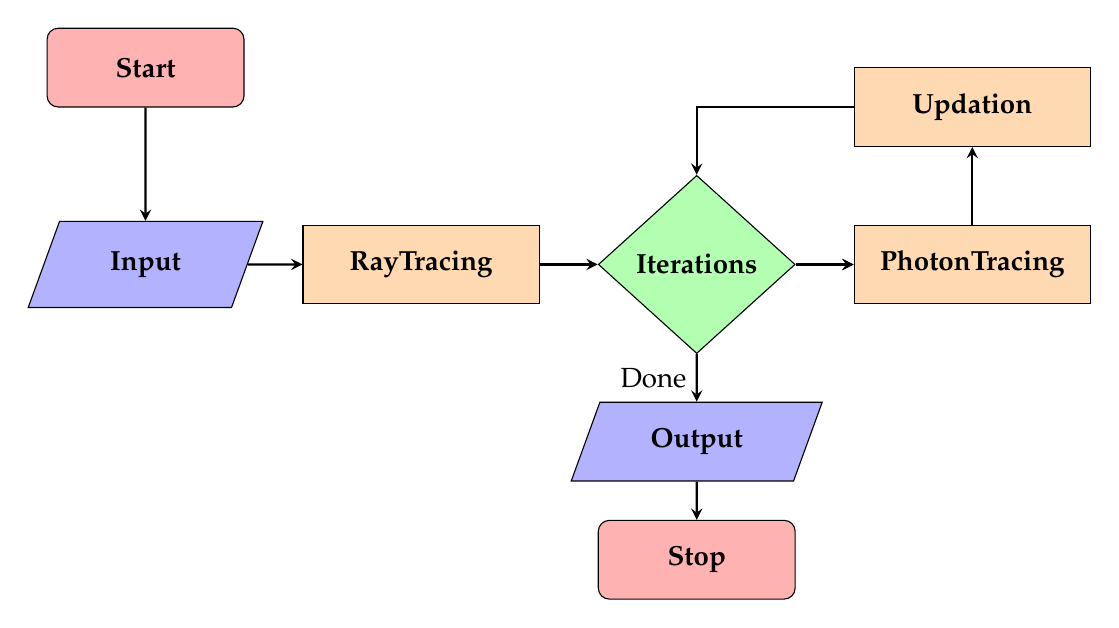
\begin{tikzpicture}[node distance=1.5cm]
\node (start) [startstop] {Start};
\node (in1) [io, below of=start, yshift=-1cm] {Input};
\node (pro1) [process, right of=in1, xshift=2cm] {RayTracing};
\node (dec1) [decision, right of=pro1, xshift=2cm] {Iterations};
\node (pro2a) [process, right of=dec1, xshift=2cm] {PhotonTracing};
\node (pro2b) [process, above of=pro2a, yshift=0.5cm] {Updation};
\node (out1) [io, below of=dec1, yshift=-0.75cm] {Output};
\node (stop) [startstop, below of=out1] {Stop};
 
\draw [arrow](start) -- (in1);
\draw [arrow](in1) -- (pro1);
\draw [arrow](pro1) -- (dec1);
\draw [arrow](dec1) -- (pro2a);
\draw [arrow](pro2a) -- (pro2b);
\draw [arrow](dec1) -- (pro2a);
\draw [arrow](dec1) -- node[left]{Done} (out1);
\draw [arrow](pro2b) -| (dec1);
\draw [arrow](out1) -- (stop);
\end{tikzpicture}}
\end{frame}

\begin{comment}
\begin{frame}
\scalebox{1}{%
\begin{algorithm}[H]
\caption{总流程}
\LinesNumbered
\KwIn{模型,材质}
\KwOut{渲染图片}
读入模型与材质信息\;
执行光线追踪,并存储撞击点\;
\For{发射光子轮数}{
    执行光子追踪\;
    存储光子图\;
    \For{撞击点}{
        找到其附近的光子\;
        累积光子对其影响\;
        更新撞击点信息\;
    }
}
生成渲染图片\;
\end{algorithm}}
\end{frame}
\end{comment}

\section{核心算法}
\subsection{Lighting Equation}
\frame{\subsectionpage}
\begin{frame}
\begin{blue}[BRDF]
BRDF(双向反射分布函数), 全称为Bidirectional Reflectance Distribution Function,%
用来定义给定入射方向上的辐射照度如何影响给定出射方向上的辐射率。%
更笼统地说,它描述了入射光线经过某个表面反射后在各个出射方向上的分布效果。
\end{blue}\pause
\begin{green}[光照方程]
\vspace{-10pt}
\begin{align}
\nonumber L_o(\mathbf{x},\omega_o)&=L_e(\mathbf{x},\omega_o)\\
&+\int_\Omega BRDF(\mathbf{x},\omega_i,%
\omega_o)L_i(\mathbf{x},\omega_i)(\omega_i\cdot\mathbf{n})\mathop{d\!}\omega_i
\end{align}\\
其中,$L_e$为直接光照,$\mathbf{x}$为空间坐标,$\mathbf{n}$为平面法向量,%
$\omega_o,\omega_i$分别为出射和入射方向。
\end{green}
\end{frame}

\subsection{Ray Tracing Pass}
\frame{\subsectionpage}
\begin{frame}
\begin{blue}[光线追踪]
从观察点出发,通过光线追踪来获得可见点(hitpoints),同时计算直接光照的贡献。
\end{blue}\pause
\begin{green}[注]
在镜面较多的场景中可用反(折)射次数作为阈值强制结束Ray Tracing Pass。
\end{green}
\end{frame}

\begin{frame}
\centering
\scalebox{0.71}{%
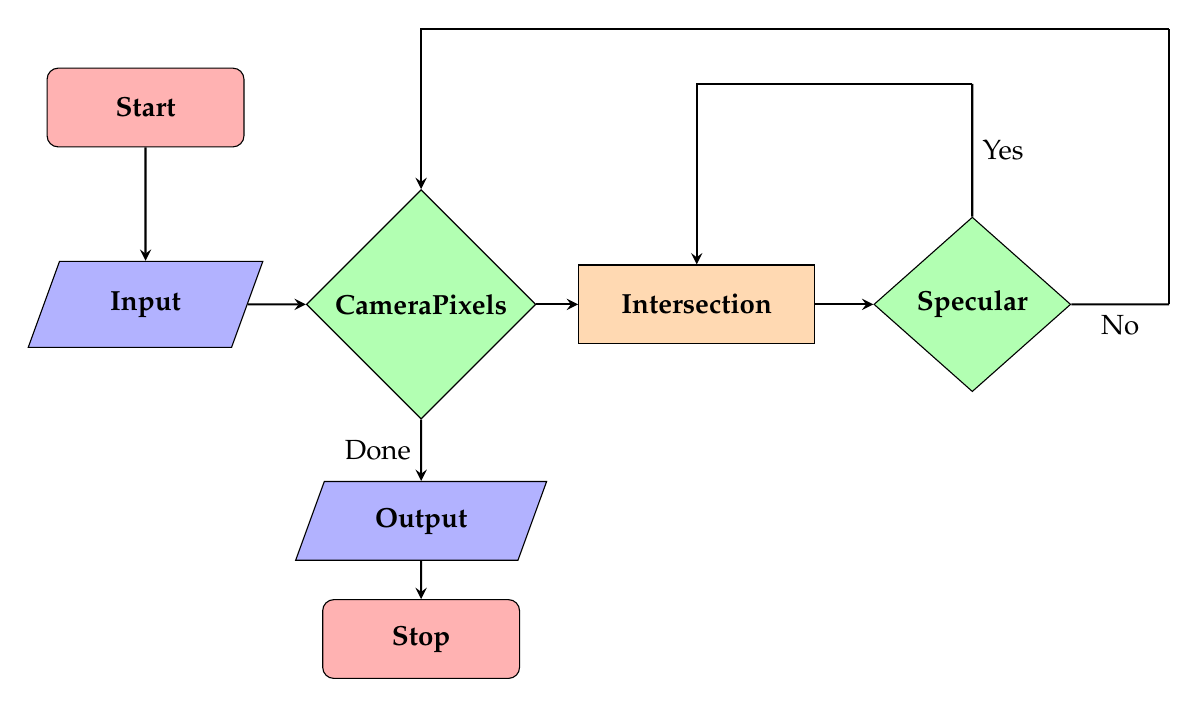
\begin{tikzpicture}[node distance=1.5cm]
\node (start) [startstop] {Start};
\node (in) [io, below of=start, yshift=-1cm] {Input};
\node (cam) [decision, right of=in, xshift=2cm] {CameraPixels};
\node (sec) [process, right of=cam, xshift=2cm] {Intersection};
\node (spe) [decision, right of=sec, xshift=2cm] {Specular};
\node (out) [io, below of=cam, yshift=-1.25cm] {Output};
\node (stop) [startstop, below of=out] {Stop};
\coordinate (p1) at (10.5cm, 0.3cm);
\coordinate (p2) at (13cm, -2.5cm);
\coordinate (p3) at (13cm, 1cm);

\draw [arrow](start) -- (in);
\draw [arrow](in) -- (cam);
\draw [arrow](cam) -- (sec);
\draw [arrow](sec) -- (spe);
\draw [line](spe) -- node[right]{Yes} (p1);
\draw [arrow](p1) -| (sec);
\draw [line](spe) -- node[below]{No} (p2);
\draw [line](p2) -- (p3);
\draw [arrow](p3) -| (cam);
\draw [arrow](cam) -- node[left]{Done} (out);
\draw [arrow](out) -- (stop);
\end{tikzpicture}}
\end{frame}

\begin{comment}
\begin{frame}
\vspace{-3pt}
\scalebox{0.9}{%
\begin{algorithm}[H]
\caption{光线追踪}
\LinesNumbered
\KwIn{摄像机,光源,宽,高,场景信息}
\KwOut{撞击点, 初始图片}
初始化图片(宽x高)\;
初始化撞击点列表\;
\For{图片像素}{
    初始化光线\;
    获取光线与场景交点\;
    \While{交点是透明材质}{
        确定是反射或折射\;
        改变光线方向\;
        重新获取交点\;
    }
    累积直接光照影响\;
    存储撞击点\;
}
返回撞击点列表和初始图片\;
\end{algorithm}}
\end{frame}
\end{comment}

\subsection{Photon Tracing Pass}
\frame{\subsectionpage}
\begin{frame}
\begin{blue}[光子追踪]
每轮Photon Tracing Pass,从光源随机方向发射一批光子,追踪每个光子的运动轨迹,%
考虑到效率,将光子能量的衰减用随机被物体表面吸收(或达到折反射阈值)来控制,%
这样每个光子的能量即为定值,折反射仅改变其颜色向量(通过BRDF计算)。
\end{blue}\pause
\begin{green}[注]
由于直接光源已在Ray Tracing Pass计算过,故每个光子与场景的第一个交点%
不必计入photon map。
\end{green}
\end{frame}

\begin{frame}
\centering
\scalebox{0.71}{%
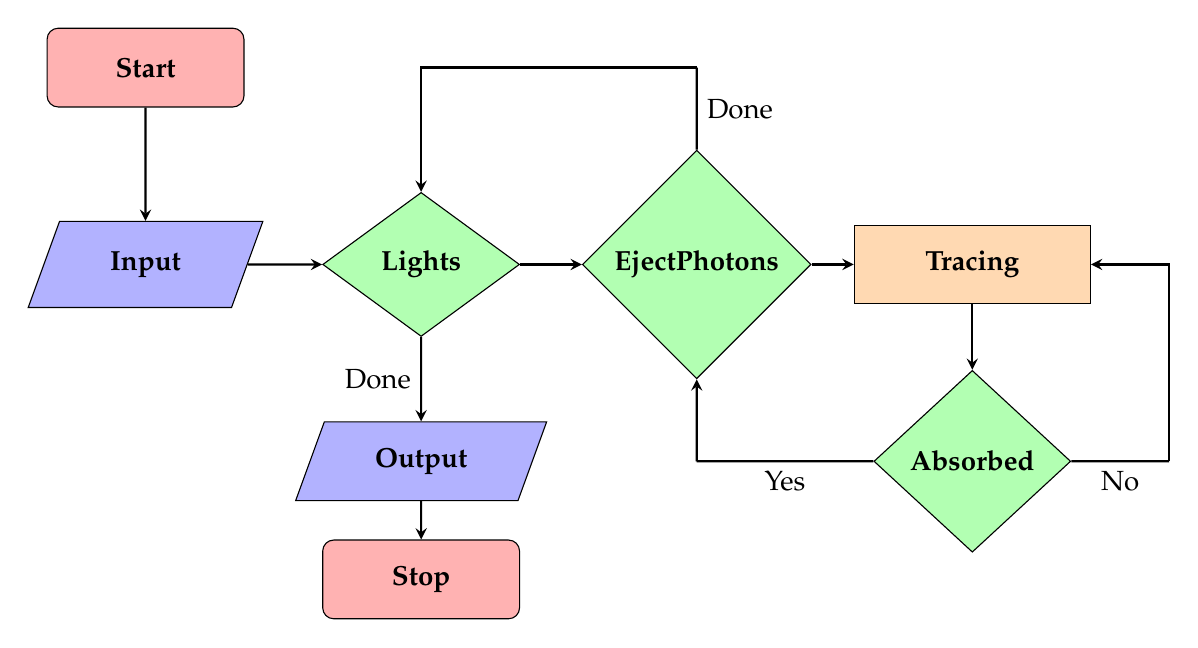
\begin{tikzpicture}[node distance=1.5cm]
\node (start) [startstop] {Start};
\node (in) [io, below of=start, yshift=-1cm] {Input};
\node (light) [decision, right of=in, xshift=2cm] {Lights};
\node (ptn) [decision, right of=light, xshift=2cm] {EjectPhotons};
\node (trc) [process, right of=ptn, xshift=2cm] {Tracing};
\node (abs) [decision, below of=trc, yshift=-1cm] {Absorbed};
\node (out) [io, below of=light, yshift=-1cm] {Output};
\node (stop) [startstop, below of=out] {Stop};
\coordinate (p1) at (13cm, -5cm);
\coordinate (p2) at (7cm, 0cm);
\coordinate (p3) at (7cm, -5cm);

\draw [arrow](start) -- (in);
\draw [arrow](in) -- (light);
\draw [arrow](light) -- (ptn);
\draw [arrow](light) -- node[left]{Done} (out);
\draw [arrow](out) -- (stop);
\draw [arrow](ptn) -- (trc);
\draw [arrow](trc) -- (abs);
\draw [line](abs) -- node[below]{Yes} (p3);
\draw [arrow](p3) -- (ptn);
\draw [line](abs) -- node[below]{No}(p1);
\draw [arrow](p1) |- (trc);
\draw [line](ptn) -- node[right]{Done} (p2);
\draw [arrow](p2) -| (light);
\end{tikzpicture}}
\end{frame}

\begin{comment}
\begin{frame}
\scalebox{1}{%
\begin{algorithm}[H]
\caption{光子追踪}
\LinesNumbered
\KwIn{光源,场景}
\KwOut{光子图}
初始化光子图\;
\For{每轮光子数量}{
    随机光子发射方向\;
    \While{未到最大折反射次数且未被吸收}{
        获取光子与场景交点\;
        将交点存储于光子图\;
        \If{光子未被吸收}{
            判断折射或反射\;
            更新方向信息\;
        }
    }
}
返回光子图\;
\end{algorithm}}
\end{frame}
\end{comment}

\subsection{Progressive Updation}
\frame{\subsectionpage}
\begin{frame}
\begin{green}[更新模型]
结束Photon Tracing Pass后,需要枚举每个hitpoint,同时统计其半径$R$内光子%
对其亮度影响。
\end{green}\pause
\begin{blue}[推导]
记$N(\mathbf{x})$为上轮后在hitpoint $\mathbf{x}$半径$R(\mathbf{x})$内的光子数,$M(\mathbf{x})$为本次新增光子数,%
同时$\hat{N}(\mathbf{x}),\hat{R}(\mathbf{x})$分别为新累计光子数和半径,则有如下更新,
\begin{gather}
\hat{N}(\mathbf{x})=N(\mathbf{x})+\alpha M(\mathbf{x})\\
\hat{R}(\mathbf{x})=R(\mathbf{x})\sqrt{\frac{N(\mathbf{x})+\alpha M(\mathbf{x})}{N(\mathbf{x})+M(\mathbf{x})}}
\end{gather}
\end{blue}
\end{frame}

\begin{frame}
\begin{blue}[推导]
记$\tau_{N}(\mathbf{x},\omega)$和$\tau_{M}(\mathbf{x},\omega)$为%
在$\mathbf{x}$处,入射光方向为$\omega$的前光强和新增光强(未乘BRDF系数),则有
\begin{equation}
\tau_{\hat{N}}(\mathbf{x},\omega)=(\tau_N(\mathbf{x},\omega)+\tau_M(\mathbf{x},\omega))%
\frac{N(\mathbf{x})+\alpha M(\mathbf{x})}{N(\mathbf{x})+M(\mathbf{x})}
\end{equation}\par
其中,$\alpha\in(0,1)$是一常数。
\end{blue}
\end{frame}

\begin{frame}
\begin{blue}[推导]
再记总发射光子数为$N_{emitted}$,$\phi$为光子光强,则最终辐照率表达式为,
\begin{align}
\nonumber L(\mathbf{x},\omega)
&=\int_{2\pi}BRDF(\mathbf{x},\omega,\omega')L(\mathbf{x},\omega')%
(\mathbf{n}\cdot\omega')\mathop(d\!)\omega'\\
\nonumber &\approx \frac{1}{\Delta A}\sum_{p=1}^{n}BRDF(\mathbf{x},\omega,%
\omega')\Delta\phi_p(\mathbf{x_p},\omega_p)\\
&=\frac{1}{\pi R(\mathbf{x})^2}\frac{\tau(\mathbf{x},\omega)}{N_{emitted}}
\end{align}
\end{blue}
\end{frame}

\section{阶段性效果图比较}
\frame{\sectionpage}
\begin{frame}
\end{frame}

\section{参考文献}
\begin{frame}[allowframebreaks]
\bibliography{EquReport}
\end{frame}

\begin{frame}
\begin{blue}[其它参考]
BRDF参数及代码来自网站\ \url{http://www.merl.com/brdf/}
png图片相关代码来自\ \url{http://lodev.org/lodepng/}
\end{blue}
\begin{green}[更多]
更多技术细节详见Equestrotopia.pdf和src文件夹中的代码\\
以及Github仓库\ \url{https://github.com/liangjs/Equestrotopia}
\end{green}
\end{frame}

\section*{Thanks}
\begin{frame}
\LARGE
\begin{beamercolorbox}[center,ht=3em]{titlelike}
\vspace{1em}
Thanks!
\end{beamercolorbox}
\end{frame}

\end{document}
